\documentclass[11pt]{report}
\usepackage{mathtools, amsthm, mathpazo, epic, eepic, color, paralist}
\usepackage{tikz}
\usepackage[margin=1in]{geometry}

\newcommand{\typo}[4]{\item Typo: on line #2 of page #1: \emph{#3} should be \emph{#4}.}
\newcommand{\funcleft}[2]{\item Example #1 on page #2.}


\begin{document}

\chapter*{APEX Section 5.4 Changes}

{\slshape Note: throughout, a positive line number refers to a line that far from the top of the page, a negative line number refers to a line that far from the bottom of the page.}

\section*{Text}

\begin{enumerate}
\item Insert the following paragraph before the first paragraph of the section:

{\slshape In this section we will find connections between differential calculus (derivatives and antiderivatives) and integral calculus (definite integrals). These connections between the major ideas of calculus are important enough to be called the Fundamental Theorem of Calculus.}

\item Replace the last paragraph before Theorem 39 with the following:

{\slshape The first part of the Fundamental Theorem of Calculus tells us how to find derivatives of these kinds of functions.}

\item Insert the following proof of Theorem 39:

{\slshape {\bfseries Proof.} In order to see why this is true, we must compute $\displaystyle\lim_{h\to 0}\frac{F(x+h)-F(x)}{h}$. Suppose $x$ and $x+h$ are in $[a,b]$. Theorem 36 implies that \[\int_a^{x+h}f(t)\,dt =\int_a^x f(t)\,dt+\int_x^{x+h} f(t)\,dt\text,\] which we can rewrite as \[\int_x^{x+h} f(t)\,dt=\int_a^{x+h} f(t)\,dt-\int_a^x f(t)\,dt.\] This allows us to simplify the denominator of the difference quotient in our limit as follows:
\begin{equation*}
\begin{split}
F(x+h)-F(x) &=\int_a^{x+h} f(t)\,dt-\int_a^x f(t)\,dt \quad\text{(by the definition of $F$)}\\
&=\int_x^{x+h} f(t)\,dt\text{,}\\
\end{split}
\end{equation*}
so we see that \[\lim_{h\to 0}\frac{F(x+h)-F(x)}{h}=\lim_{h\to 0}\frac 1h\int_x^{x+h} f(t)\,dt.\]

Assume for the moment that $h>0$. Since $x$ and $x+h$ are both in $[a,b]$ and $f$ is continuous on $[a,b]$, $f$ is also continuous on $[x,x+h]$. Applying the Extreme Value Theorem (Theorem 25), we know that $f$ must have an absolute minimum value $f(u)=m$ and an absolute maximum value $f(v)=M$ on this interval. In other words, $m\leq f(t)\leq M$ whenever $x\leq t\leq x+h$. Using the Comparison Properties of Integrals, we can now say that \[\int_x^{x+h} m\,dt \leq \int_x^{x+h} f(t)\,dt \leq \int_x^{x+h} M\,dt.\] Computing the outer integrals, this becomes 
\begin{equation*}
\begin{split}
m(x+h-x)\leq \int_x^{x+h} f(t)&\,dt \leq M(x+h-x)\text{,\quad or}\\
mh\leq \int_x^{x+h} f(t)&\,dt \leq Mh.\\
\end{split}
\end{equation*}
Since $h>0$, we may divide by $h$ to obtain \[f(u)=m\leq \frac1h\int_x^{x+h} f(t)\,dt \leq M=f(v).\]

Now suppose that $h<0$. Proceding as before, we know that $f$ has an absolute minimum value $f(u)=m$ and an absolute maximum value $f(v)=M$ on the interval $[x+h,x]$. We know that $m\leq f(t)\leq M$ whenever $x+h\leq t\leq x$, so we have \[\int_{x+h}^x m\,dt\leq\int_{x+h}^x f(t)\,dt\leq \int_{x+h}^x M\,dt.\] Once again we compute to obtain \[ -mh\leq \int_{x+h}^x f(t)\,dt \leq -Mh.\]
Since $-h>0$, we can divide by $-h$ to obtain:
\begin{equation*}
\begin{split}
m\leq -\frac1h\int_{x+h}^x f(t)&\,dt \leq M\\
f(u)=m\leq \frac1h \int_x^{x+h} f(t)&\,dt \leq M=f(v)\quad\text{(using Theorem 36(2))}\\
\end{split}
\end{equation*}

We are now ready to compute the desired limit, \[\lim_{h\to 0}\frac{F(x+h)-F(x)}{h}=\lim_{h\to 0}\frac1h\int_x^{x+h} f(t)\,dt.\] Whether $h>0$ or $h<0$, we know that \[f(u)\leq \frac1h\int_x^{x+h} f(t)\,dt\leq f(v)\text{,}\] where $u$ and $v$ are both between $x$ and $x+h$. Note that 
\[\lim_{h\to 0} (x+h)=x \text{\quad and \quad} \lim_{h\to 0} x=x\text{,}\] so the Squeeze Theorem (Theorem 4) says that \[\lim_{h\to 0}u=x \text{\quad and \quad} \lim_{h\to 0} v=x.\] Since $f$ is continuous at $x$, we know that \[\lim_{h\to 0} f(u)=f(x)\text{\quad and \quad} \lim_{h\to 0}f(v)=f(x).\]  Finally, we know that \[f(u)\leq \frac1h \int_x^{x+h} f(t)\,dt\leq f(v)\text{,}\] so applying the Squeeze Theorem again tells us that \[\lim_{h\to 0}\frac1h\int_x^{x+h} f(t)\,dt=f(x).\] 

Therefore $F'(x)=f(x)$ as desired. \qedsymbol}

\item We talked about inserting a proof for both parts of the Fundamental Theorem, but there is already a proof for part 2. It just occurs before the statement.

\item Delete the subsection on the area between curves on pages 233-234.


\item Insert the following proof of Theorem 42:

{\slshape {\bfseries Proof.} If $a=b$, then $\int_a^a f(x)\,dx =0=f(a)(a-a)$. Otherwise, we define the following for $x$ in $[a,b]$: \[ F(x)=\int_a^x f(t)\,dt.\] Applying Theorem 39 we know that $F$ is differentiable on $[a,b]$ and that $F'(x)=f(x)$ for any $x$ in $[a,b]$. We may now apply the Mean Value Theorem for Differentiation (Theorem 27) to see that there is a value $c$ in $(a,b)$ such that \[F'(c)=\frac{F(b)-F(a)}{b-a}.\] Note that $F'(c)=f(c)$ and that $F(b)-F(a)=\int_a^b f(x)\,dx$ by Theorem 40. Therefore we can rewrite our equation as: 
\begin{equation*}
\begin{split}
f(c)&=\frac{\int_a^b f(x)\,dx}{b-a}\text{, or}\\
f(c)(b-a)&=\int_a^b f(x)\,dx.\\
\end{split}
\end{equation*}
\qedsymbol
}

\item On page 237, beginning on line -5, replace \emph{The next chapter is devoted to} with \emph{Much of our time in Calculus II will be devoted to}


\end{enumerate}


\section*{Problems}
\begin{enumerate}

\item In the instructions for current problem section 5-28, change the instructions to \emph{use the Fundamental Theorem of Calculus Part 2 to evaluate the definite integral:}

\item In the instructions for current problem section 53-56, change the instructions to \emph{use the Fundamental Theorem of Calculus Part 1 to find $F'(x)$:}

\item Delete problems 49-52.

\item Add the following problem: Let $g(x)=\int_0^x f(t)\,dt$ where $f$ is the function whose graph is shown below.
\begin{enumerate}
\item Evaluate $g(x)$ for $x=0,1,2,3,4,5,6$.
\item Estimate $g(7)$.
\item Where does $g$ have a minimum value? a maximum value?
\item Sketch the graph of $g$.
\end{enumerate}

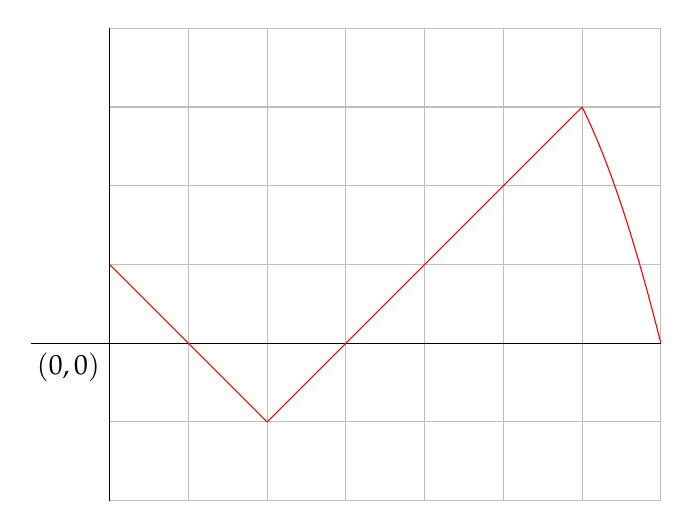
\begin{tikzpicture} [smooth]
   \draw [color=lightgray] (0,-2) grid (7,4);
   \draw (-1,0) -- (7,0);
   \draw (0,-2) -- (0,0);
   \draw (0,0) node [anchor=north east] {$(0,0)$} -- (0,4);
   \draw [color=red, domain=0:2] plot(\x, {1-\x});
   \draw [color=red, domain=2:6] plot(\x, {\x-3});
   \draw [color=red, domain=6:7] plot(\x, {-\x*\x+10*\x-21});
\end{tikzpicture}

\end{enumerate}

\end{document}
